\documentclass{sigchi}

% Use this section to set the ACM copyright statement (e.g. for
% preprints).  Consult the conference website for the camera-ready
% copyright statement.

% Copyright
\CopyrightYear{2020}
%\setcopyright{acmcopyright}
\setcopyright{acmlicensed}
%\setcopyright{rightsretained}
%\setcopyright{usgov}
%\setcopyright{usgovmixed}
%\setcopyright{cagov}
%\setcopyright{cagovmixed}
% DOI
\doi{https://doi.org/10.1145/3313831.XXXXXXX}
% ISBN
\isbn{978-1-4503-6708-0/20/04}
%Conference
\conferenceinfo{CHI'20,}{April  25--30, 2020, Honolulu, HI, USA}
%Price
\acmPrice{\$15.00}

% Use this command to override the default ACM copyright statement
% (e.g. for preprints).  Consult the conference website for the
% camera-ready copyright statement.

%% HOW TO OVERRIDE THE DEFAULT COPYRIGHT STRIP --
%% Please note you need to make sure the copy for your specific
%% license is used here!
% \toappear{
% Permission to make digital or hard copies of all or part of this work
% for personal or classroom use is granted without fee provided that
% copies are not made or distributed for profit or commercial advantage
% and that copies bear this notice and the full citation on the first
% page. Copyrights for components of this work owned by others than ACM
% must be honored. Abstracting with credit is permitted. To copy
% otherwise, or republish, to post on servers or to redistribute to
% lists, requires prior specific permission and/or a fee. Request
% permissions from \href{mailto:Permissions@acm.org}{Permissions@acm.org}. \\
% \emph{CHI '16},  May 07--12, 2016, San Jose, CA, USA \\
% ACM xxx-x-xxxx-xxxx-x/xx/xx\ldots \$15.00 \\
% DOI: \url{http://dx.doi.org/xx.xxxx/xxxxxxx.xxxxxxx}
% }

% Arabic page numbers for submission.  Remove this line to eliminate
% page numbers for the camera ready copy
% \pagenumbering{arabic}

% Load basic packages
\usepackage{balance}       % to better equalize the last page
\usepackage{graphics}      % for EPS, load graphicx instead 
\usepackage[T1]{fontenc}   % for umlauts and other diaeresis
\usepackage{txfonts}
\usepackage{mathptmx}
\usepackage[pdflang={en-US},pdftex]{hyperref}
\usepackage{color}
\usepackage{booktabs}
\usepackage{textcomp}
\usepackage{graphicx}

% Some optional stuff you might like/need.
\usepackage{microtype}        % Improved Tracking and Kerning
% \usepackage[all]{hypcap}    % Fixes bug in hyperref caption linking
\usepackage{ccicons}          % Cite your images correctly!
% \usepackage[utf8]{inputenc} % for a UTF8 editor only

% If you want to use todo notes, marginpars etc. during creation of
% your draft document, you have to enable the "chi_draft" option for
% the document class. To do this, change the very first line to:
% "\documentclass[chi_draft]{sigchi}". You can then place todo notes
% by using the "\todo{...}"  command. Make sure to disable the draft
% option again before submitting your final document.
\usepackage{todonotes}

% Paper metadata (use plain text, for PDF inclusion and later
% re-using, if desired).  Use \emtpyauthor when submitting for review
% so you remain anonymous.
\def\plaintitle{Promoting Health Using VR/AR}
\def\plainauthor{Aaron Marquez, Adan Soto, Antony Smelianski, Trevon Donsereaux}
\def\emptyauthor{}
\def\plainkeywords{Virtual reality; physical activity; heart rate; oculus quest}
\def\plaingeneralterms{Documentation, Standardization}

% llt: Define a global style for URLs, rather that the default one
\makeatletter
\def\url@leostyle{%
  \@ifundefined{selectfont}{
    \def\UrlFont{\sf}
  }{
    \def\UrlFont{\small\bf\ttfamily}
  }}
\makeatother
\urlstyle{leo}

% To make various LaTeX processors do the right thing with page size.
\def\pprw{8.5in}
\def\pprh{11in}
\special{papersize=\pprw,\pprh}
\setlength{\paperwidth}{\pprw}
\setlength{\paperheight}{\pprh}
\setlength{\pdfpagewidth}{\pprw}
\setlength{\pdfpageheight}{\pprh}

% Make sure hyperref comes last of your loaded packages, to give it a
% fighting chance of not being over-written, since its job is to
% redefine many LaTeX commands.
\definecolor{linkColor}{RGB}{6,125,233}
\hypersetup{%
  pdftitle={\plaintitle},
% Use \plainauthor for final version.
%  pdfauthor={\plainauthor},
  pdfauthor={\emptyauthor},
  pdfkeywords={\plainkeywords},
  pdfdisplaydoctitle=true, % For Accessibility
  bookmarksnumbered,
  pdfstartview={FitH},
  colorlinks,
  citecolor=black,
  filecolor=black,
  linkcolor=black,
  urlcolor=linkColor,
  breaklinks=true,
  hypertexnames=false
}

% create a shortcut to typeset table headings
% \newcommand\tabhead[1]{\small\textbf{#1}}

% End of preamble. Here it comes the document.
\begin{document}

\title{\plaintitle}

\numberofauthors{4}
\author{
  \alignauthor{Aaron Marquez\\
    \affaddr{Colorado State University}\\
    \affaddr{Fort Collins, Colorado}\\
    \email{azmarque@rams.colostate.edu}}\\
  \alignauthor{Adan Soto\\
    \affaddr{Colorado State University}\\
    \affaddr{Fort Collins, Colorado}\\
    \email{asoto98@rams.colostate.edu}}\\
  \alignauthor{Antony Smelianski\\
    \affaddr{Colorado State University}\\
    \affaddr{Fort Collins, Colorado}\\
    \email{asmelian@rams.colostate.edu}}\\
  \alignauthor{Trevon Donsereaux\\
    \affaddr{Colorado State University}\\
    \affaddr{Fort Collins, Colorado}\\
    \email{tdons@rams.colostate.edu}}\\
}

\maketitle

% ACM Classfication
\begin{CCSXML}
<ccs2012>
<concept>
<concept_id>10003120.10003121.10003124.10010866</concept_id>
<concept_desc>Human-centered computing~Virtual reality</concept_desc>
<concept_significance>500</concept_significance>
</concept>
</ccs2012>
\end{CCSXML}

\ccsdesc[500]{Human-centered computing~Virtual reality}
\ccsdesc[300]{Human-centered computing~User Studies}

% Author Keywords
\keywords{\plainkeywords}

% Print the classficiation codes, codes @ https://dl.acm.org/ccs/ccs_flat.cfm
\printccsdesc

\section{Introduction}

Given the increase in obesity and the common lack of physical activity among Americans and people of the world, we have decided to develop a project that aims to tackle this problem by giving users the opportunity to exercise at any given time while making it seem like a videogame. This is so that the feeling of playing a videogame makes the user forget the fact that they are working out. In order to facilitate the interest of exercise through gaming our project has to be interesting and engaging enough to get people to actually partake in the game. By using newer technologies like VR, the goal is to bring enough interest/wow factor by users to actually pursue trying the game. We plan on using the technologies described in the next section. With these technologies we can create many different athletic activities that users can partake in to play a specific skill they wish to improve on. The goal is to make it as close to real life as possible but with the limitation of current technologies it won’t feel life like just yet. 

\subsection{Literature Review}

\subsubsection{Research on Application of Virtual Reality Technology in Competitive Sports}

The Research on Application of Virtual Reality Technology in Competitive Sports journal article\cite{sanz_franck_lecuyer_anatole_ferran_2015} focuses on the potential of Virtual Reality to improve the ability of professional athletes to train harder and more than usual and take their skills to a higher level. It focuses on the important aspects that must be perfected in order for Virtual Reality to be effective as a proper training method. It emphasizes the importance of having accurate opponents with real techniques and strategies as well as mimicking real environments in order for the training. If these factors are correct there is a great benefit that can come from using Virtual Reality technology as another tool in a coach’s toolbox to further develop athletes’ abilities. Although this research might not be directly related to the research being conducted in this paper, it still brings up some relevant issues that must be addressed further into the developing stage, this being the importance of creating an immersive environment. The main focus of the article was taking training and athletes to a higher level and also having the ability to record many different sorts of physiologic and biologic data while they train. Perhaps biologic and physiologic data are not the main focus of this research paper but escalating skill and introducing participants to a specific sport are definitely of interest. The Research on Application of Virtual Reality Technology in Competitive Sports journal article definitely helps pointing this research paper in the right direction by proving many of the factors that make VR appropriate for athletes that can also translate to beginner participants. It also shows that what this research paper and experiment are trying to accomplish are things that are applicable for the general public and of interest to the competitive sports industry.

\subsubsection{VR to improve Sports Performance}

The usage of Virtual reality in a sports environment provides many benefits to athletes by creating different environment’s that players can experience based on what they are trying to improve on.  The key components of virtual reality provide 3 illusions, place illusion, plausible illusion and embodiment. With these athletes are able to completely immerse themselves in stressful situations similar to game conditions and can work on movements, judgements and predictability to improve them while certain brain stimuli are working. This is currently being developed further for NFL players allowing them to practice plays on a field while they are home and soccer players to help with reaction time and predictability of ball movement. 
With these improvements lots of growth can be seen through VR specifically the recovery aspect for players or even normal people at home. If a player suffers an injury, they can still place themselves in those environments to prevent the loss of skill during recovery and can get them back on the field at full capacity. People at home can learn certain exercises at home and still be able to show up to athletic events, clubs, and gyms without the fear of not knowing what they are doing.\cite{barca_innovation_hub_2019}

\subsubsection{Introducing Competitive Anxiety and Pressure in VR Sport Training}

Introducing Competitive Anxiety and Pressure in VR Sports Training journal’s\cite{wang_2012} focal point is proposing methodological guidelines for designing sport training scenarios concerning both the training routine they must have like replicating anxiety situations an athlete can have for example, a free throw to win the game, and external factors the might influence the athlete including audience, and athlete's expectations. The researchers designed an experiment setup that reproduced a 10 m olympic shooting event. They analyzed whether changes in environment induce changes in the user performance, and the subjective perception of the task. This environment included stressors the participant might endure in real life like an aggressive audience, or unforced errors. The results showed significant differences in the physiological and behavioral data, and also in their subjective impressions. Overall the results suggested that the highly immersive systems could be used for training athletes. This could help our experiment as this application is to promote health to the regular person, but people like being able to “train and feel like a professional athlete”. This helped us understand that users want a realistic feeling. By having a realistic feeling the users will enjoy the game more, and will most likely play it more often, which results in a higher activity level.

\subsubsection{Active Video Games to Promote Physical Activity in Children and Youth}

The Active Video Games to Promote Physical Activity in Children and Youth article\cite{biddiss_2010} focuses on how physical inactivity in youth is a health issue that may only be solved through an approach of adding attractive opportunities for daily physical activity. One way to increase children’s motivation to be active is through active video games(AVG). With new advancements in the virtual reality field, AVG can be seen as an exciting way to stay active for children. This article looks at other studies that were conducted and analyzes the data. One of the key findings from a few points in the data was that AVG often raises heart rates, but that AVG provides light to moderate physical activity for its users. Between children and adults, activity intensity varies based on the game and is greater in games that involve more lower body movements. The article also notes that more research is needed to help strengthen evidence for AVG to promote more physical activity. This project is set up in hopes of adding more supporting evidence. Though it is not geared towards testing the children, it will focus on young adults of varying physical backgrounds. The center of attention will be on heart rates and user satisfaction to help gain evidence that VR can be used to promote physical activity amongst young adults.

\section{Idea of prototype}

The first prototype will be a working game developed in unity for use with an Oculus Quest. A very simple design can be seen in figure 1. It will allow the user to move around within the game. Such movements include walking, ducking, and jumping. This prototype will include a very basic setting, but will be later updated in another iteration of the game. Another feature that may or may not be implemented in the first prototype is objects being thrown towards the user like the red balls shown in figure 1. Some more features for future iterations include a score HUD, timer, and other basic movements for the user.  

\begin{figure}
    \centering
    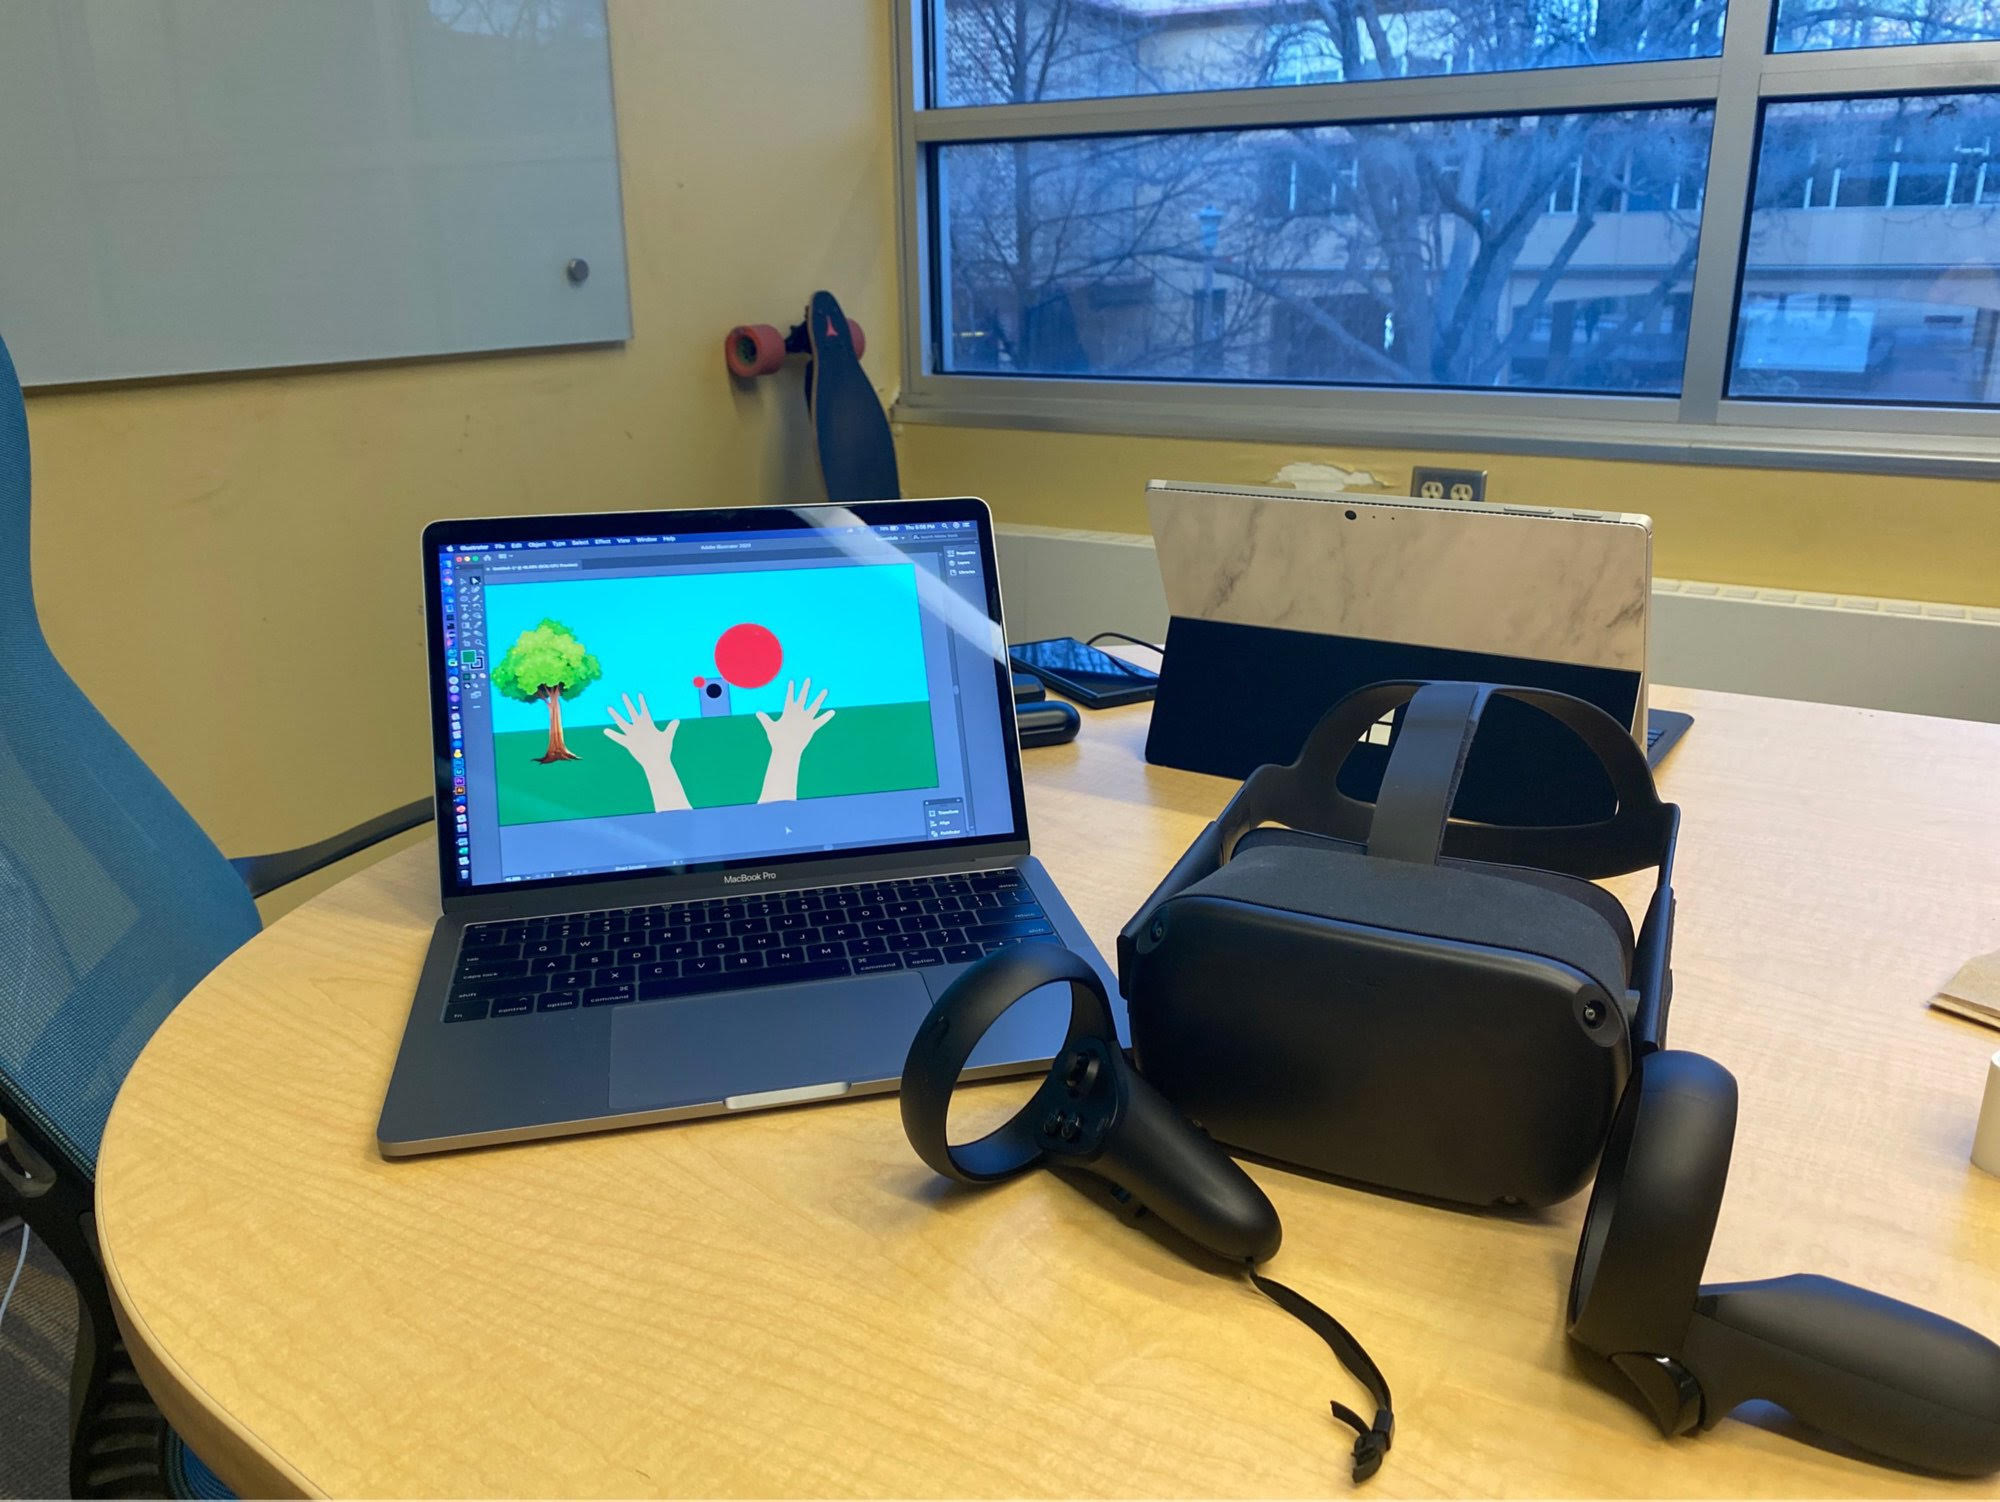
\includegraphics[scale=0.10]{figures/HCIPrototype.jpg}
    \caption{Current design for prototype}
    \label{fig:my_label}
\end{figure}

\section{Draft Design of Experiment}

\subsection{Variables}
Independent Variable: setting(VR vs Real life), Fitness level of Participants, Age\\
Dependent Variable: Heart rate, user satisfaction\\
Random Variables: Temperature, Speed of ball\\
Control Variables: VR headset, Instructions, Athleticism of the participant

\subsection{Participants}

Participants will be college students with different levels of activity. Participants will be recruited from a groups of friends, fraternities, and students in the Computer Science program. The idea is to have people who have differing levels of interest in sports and exercise as well as different human characteristics. 

\subsection{Task}

A task that will test the enjoyment and likelihood of performing a certain sport/activity in two different settings to see if VR is a liable option to introduce a different range of people into sports is the main goal. The task will require participants to complete a session of dodgeball outdoors where the participants will have to dodge balls with different moves which will be required in order to assess intensity of workout, this task will be performed outdoors in real life as well as in VR to test the enjoyment and likelihood of repeating the exercise. A range of variables will be measured and recorded in order to more accurately come to a valid conclusion that takes independent, dependent, random, and controlled variables into consideration.


\balance{}

\balance{}

% REFERENCES FORMAT
% References must be the same font size as other body text.
\bibliographystyle{SIGCHI-Reference-Format}
\bibliography{sample}

\end{document}

%%% Local Variables:
%%% mode: latex
%%% TeX-master: t
%%% End:
